%*************************************************************
\chapter{Scribbler}\label{ch:scribbler}
%*************************************************************

In den vergangenen Kapitel zeigten wir mit etlichen Beispielen wie und mit welchen Hilfsmitteln Gruppenmeetings abgehalten werden können. Sind es traditionelle Medien wie Papier und Filpcharts, oder elektronische Medien wie computerunterstützte Whiteboardsysteme - sie alle finden Einsatz in Designsessions und bieten verschiedenste Vor- und Nachteile.

\medskip Im Folgenden wollen wir \emph{Scribbler} vorstellen, ein elektronisches Interface, das die kollaborative Arbeit an virtuellen Artefakten unterstützen soll. Ähnlich wie die Autoren der bereits im ersten Kapitel beschriebenen Systeme, versuchten wir ein System zu kreieren, das die beiden Design-Arbeitswelten - geprägt durch traditionelle und elektronische Medien - mit einander verbindet und ihre Vorteile herausarbeitet. Im Gegensatz zu den bisherigen Ansätzen jedoch, ist \emph{Scribbler} ein elektronisches Skizziersystem, welches ein barrierefreies Arbeiten ermöglicht.

\medskip Um dies zu zeigen, wollen wir vorerst, nach einer kurzen Beschreibung unserer Ausgangsituation, die Anforderungen eines kollaborativen Skizziersystems, die wir durch unsere Literaturrecherche gesammelt haben, zusammengefasst präsentieren. Danach werden wir die Vorgehensweise zur Erstellung unseres Prototyps schildern, welche selbst einige Designmethoden aus \autoref{ch:designTheorie} beinhaltet. Anschließend präsentieren wir die simple Oberfläche von \emph{Scribbler} und dessen Funktionsumfang mit technischen Hintergründen. Zu guter Letzt stellen wir die Anforderungen und Merkmale gegenüber und beschreiben gewonnene Erkenntnisse aus Benutzererfahrungen.

\section{Ausgangsituation \& Rahmenbedingungen}
Die Technisierung vieler Berufe führte dazu, dass gewisse Arbeitsgegenstände ein elektronisches Abbild bekamen. Grafikdesigner beispielsweise fertigen heutzutage Präsentationszeichnungen, im Gegensatz zu früher, digital an. Neuere Berufsparten wie Interfacedesign setzen die tagtägliche Arbeit mit digitalen Artefakten vorraus. Wie schon in den vorigen Kapitel erwähnt, ist (im Besonderen) Design eine kollaborative Tätigkeit, wofür sich Gruppen zu Meetings treffen um gemeinsam neue Lösungen zu erarbeiten. Ein bewährtes und wichtiges Instrument dazu sind Stifte zur Erstellung von Skizzen, um Gedanken zu manifestieren.\\
Ein wesentlicher Bestandteil moderner Meetingräume ist ein zentraler Bildschirm oder Projektor, der als Präsentationsmittel verwendet wird. Zudem ist meistens eine Zeichenfläche vorhanden, wie z.B. Whiteboards oder Flip-Charts, um kollaborativ erarbeitete Ideen festzuhalten und neue Ideen zu explorieren.

\medskip Das Institut für Gestaltungs- und Wirkungsforschung an der TU Wien verfügt über so einen Meetingraum. Er besteht aus mehreren Tischen, die in der Mitte des Raumes zusammen gestellt wurden und um denen sich Sitzmöglichkeiten befinden. Neben einem Flip-Chart befindet sich ein {52\dq} großer Bildschirm in der Mitte einer Wand, auf den alle Meetingteilnehmer, von ihren Sitzplätzen aus, blicken können. Mit dem Screen ist ein Computer (Apple Mac Mini) verbunden, auf den Daten über ein drahtlos Netzwerk gespielt werden können. Eine zusätzliche drahtlose Tastatur und Maus ermöglichen eine bequeme Steuerung. Zusätzliche Peripherie kann auf der Hinterseite des Computers angeschlossen werden.

\medskip Das Kerngebiet des Instituts ist \ac{HCI}, wodurch der Meetingraum oft dazu verwendet wird, Designs für interaktive Systeme, Applikationen oder Webinhalte zu erarbeiten. Ein Problem, das dabei erwartungsgemäß entsteht ist, dass bereits umgesetzte Inhalte nur digital vorhanden sind, was den Einsatz der wichtigsten Designmethode - Skizzieren - auf dem Artefakt fast unmöglich macht. Ziel unserer Arbeit war es nun ein Tool zu entwickeln, das es erlaubt, auf jegliche präsentierte Inhalte - seien es Webseiten, Programmoberflächen oder Bilder - >>kritzeln<< zu können. \emph{Scribbler} soll so die Barriere zwischen der realen Welt und der digitalen Welt aufbrechen.

\section{Anforderungen eines kollaborativen Skizziersystems}
Die letzten Kapitel gaben Aufschluss über das Verbesserungspotential vieler existierender Systeme. Wichtige literarische Größen auf diesem Gebiet, wie z.B. Lee, Olsen, Tang, Larsson, Johnson oder Prante, wiesen auf wesentliche Erkenntnisse hin, die ein solches System formen. Diese Erkenntnisse können vier großen Einflussfaktoren zugeordnet werden: \emph{Hardware}, \emph{Software}, \emph{Kollaboration} und \emph{Skizzieren}. \autoref{fig:kollaborativesSkizziersystem} zeigt eine Aufstellung dieser Erkenntnisse, in Verbindung zu ihren Einflussfaktoren.

\begin{figure}
	        {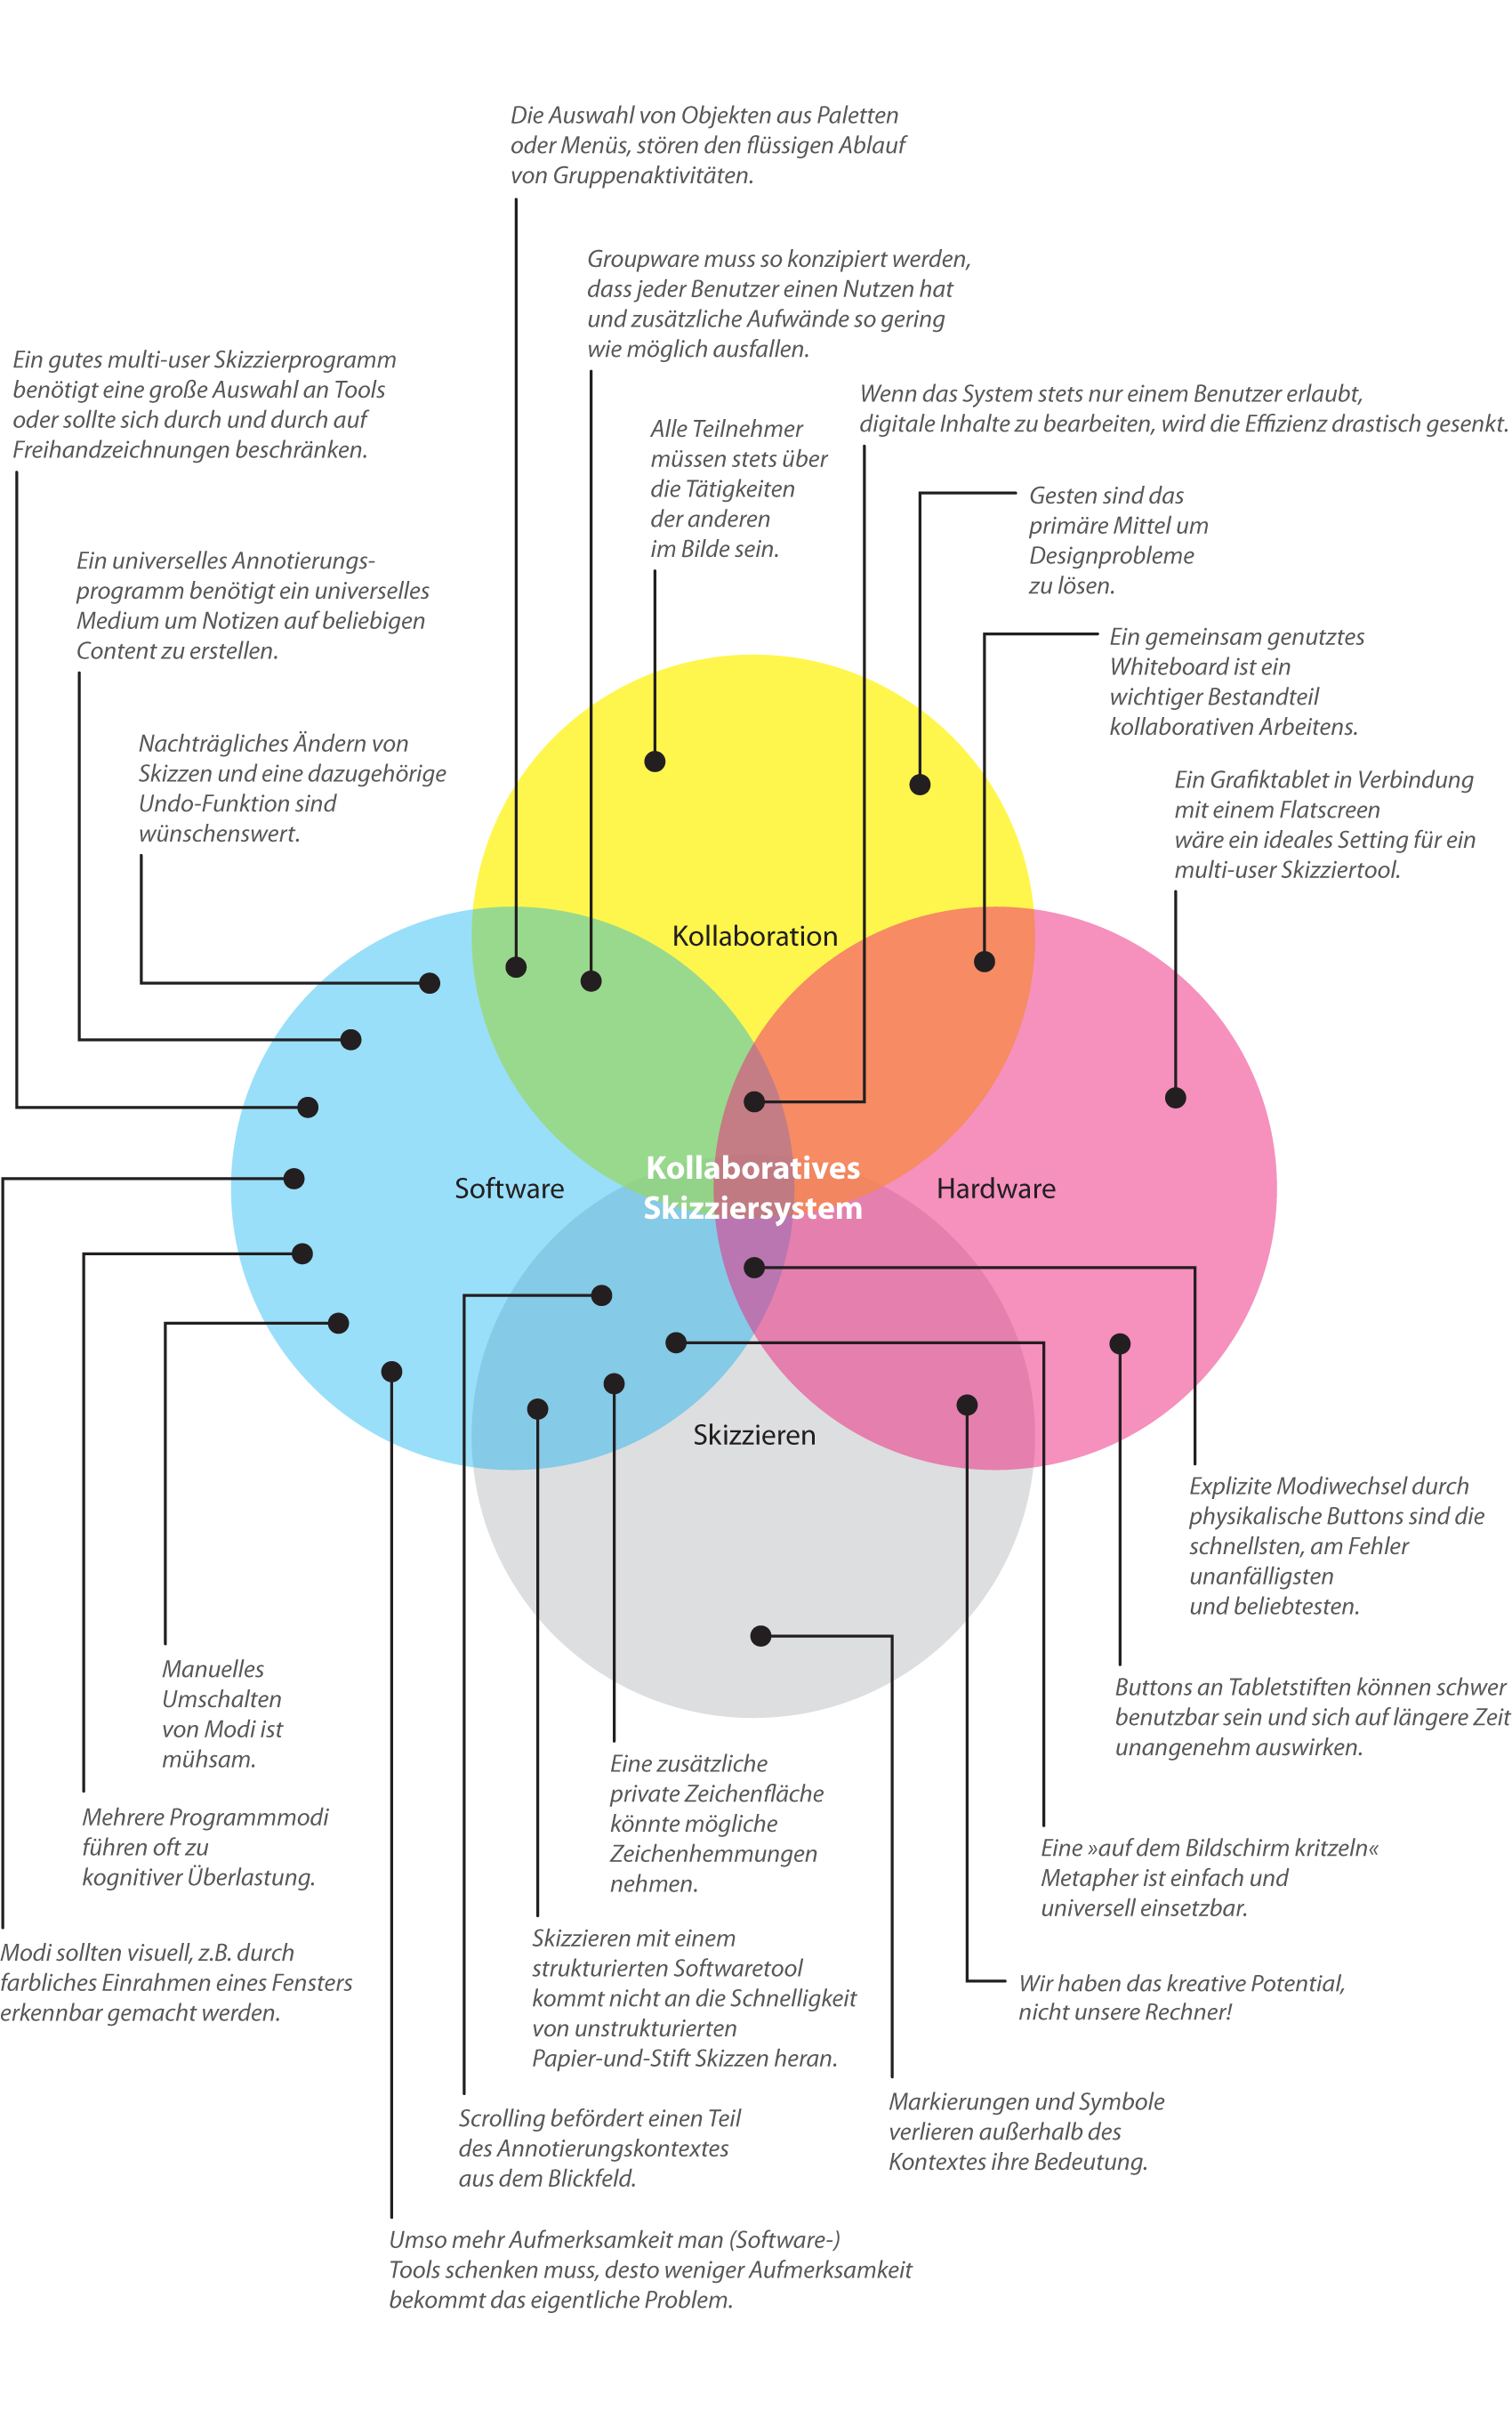
\includegraphics[bb=0cm 0cm 14.39cm 23.01cm]{gfx/kollaborativesSkizziersystem}}
		\caption[Anforderungen eines kollaborativen Skizzersystems]{Anforderungen eines kollaborativen Skizzersystems, bestehend aus den vier Einflussfaktoren: Hardware, Software, Kollaboration \& Skizzieren.}\label{fig:kollaborativesSkizziersystem}
\end{figure}

\medskip \emph{Hardware} Ein ideales Setting für ein kollaboratives Skizziertool wäre laut Lee ein Grafiktablet in Verbindung mit einem Flatscreen. Dies wäre die bestmöglichste Annäherung zu einer Technologie, die Stift und Papier ersetzen könnte. Sie würde ebenso zur Umsetzung eines Whiteboard Systems beitragen, was einen wichtigen Bestandteil kollaborativen Arbeitens ausmacht. Buttons an Tabletstiften können schwer benutzbar sein und sich auf längere Zeit unangenehm auswirken, deswegen sollte davon abgeraten werden diese mit einer Funktion zu belegen. 

\medskip \emph{Software} Ein gutes multi-user Skizzierprogramm benötigt eine große Auswahl an Tools, oder sollte sich durch und durch auf Freihandzeichnungen beschränken. Welcher Ansatz besser funktioniert, müsse laut Lee ausprobiert werden. Klar ist jedoch, dass umso mehr Aufmerksamkeit einem Softwaretool geschenkt werden muss, desto weniger Aufmerksamkeit bekommt das eigentliche Problem. Deswegen sollte solch ein System so simpel wie möglich aufgebaut sein. \\
Will man beispielsweise mehrere Programmmodi verwenden, muss man sich vor Augen führen, dass diese oft zur kognitiven Überlastung führen. Aus diesem Grund sollte der aktuelle Modus visuell, z.B. durch farbliches Einrahmen eines Fensters, erkennbar gemacht werden. Zudem ist das manuelle Umschalten von Modi mühsam. Es hat sich jedoch herausgestellt, dass explizite Modiwechsel durch physikalische Buttons, die schnellsten, am Fehler unanfälligsten und beliebtesten sind. \\
Will man ein universelles Annotierungstool schaffen, das über alle verwendeten Programme eines Benutzers funktioniert, benötigt man auch ein universelles Medium um Notizen auf beliebigen Content zu erstellen. Außerdem sind das nachträgliche Ändern von Skizzen und eine dazugehörige Undo-Funktion wünschenswert.

\medskip \emph{Kollaboration} Gemeinsam genutzte Systeme müssen so konzipiert werden, dass jeder Teilnehmer einen Nutzen hat. Wenn das System nur einen Benutzer erlaubt, digitale Inhalte zu bearbeiten, wird die Effizienz drastisch gesenkt. Zusätzliche Aufwände sollten so gering wie möglich ausfallen. Die Auswahl von Objekten aus Paletten oder Menüs, stören beispielsweise den flüssigen Ablauf von Gruppenaktivitäten. Die Teilnehmer der Kollaboration sollten ebenso stets über die Tätigkeiten der anderen im Bilde sein. Gesten spielen dabei eine wichtige Rolle.

\medskip \emph{Skizzieren} Das Zeichnen mit einem strukturierten Softwaretool kommt nicht an die Schnelligkeit von unstrukturierten Papier- und-Stift Skizzen heran. Eine >>auf dem Bildschirm kritzeln<< Metapher ist somit einfach und universell einsetzbar. Skizzen verlieren außerhalb des Kontextes ihre Bedeutung. Somit muss darauf geachtet werden, dass der Kontext stets bewahrt wird. Scrolling befördert z.B. einen Teil des Annotierungskontextes aus dem Blickfeld und benötigt somit zusätzliche Aufmerksamkeit bei der Umsetzung. Zudem könnte eine zusätzliche private Zeichenfläche mögliche Zeichenhemmungen von Teilnehmern nehmen. Alles in Allem haben wir das kreative Potential - ein Skizziersystem muss sich entsprechend adaptieren können.

\section{Vorgehensweise}

\subsection{Recherche}
\subsection{Skizzieren}
\subsection{Prototyping}
\subsection{User Testing}

\section{Scribbler at a Glance}

\subsection{Technik}
\begin{lstlisting}[float,caption=A scribbler code snippet]
for i:=maxint to 0 do
begin
{ do nothing }
end;
\end{lstlisting}

\subsection{GUI Design}

\section{User Review}

\section{Acievements}

\section*{Zusammenfassung}
lorem ipsum